\chapter{Technical Background}
\label{chapter:background}

This chapter establishes the scientific and technical foundation for the screening system presented in this report. It begins by defining \ab{mtbi} and the pathological mechanisms that make it difficult to detect with conventional imaging (\Cref{sec:bg-mtbi}). It then reviews existing diagnostic approaches, evaluating each against the screening requirements established in \Cref{chapter:introduction} to justify the choice of automated pupillometry (\Cref{sec:bg-existing}), before detailing the oculomotor biomarkers that underpin the system design (\Cref{sec:bg-oculomotor}). Finally, it surveys prior engineering work on automated oculomotor assessment (\Cref{sec:bg-engineering}).

\section{Mild Traumatic Brain Injury}
\label{sec:bg-mtbi}

\ab{mtbi}, also known as concussion, is defined by the 2023 American Congress of Rehabilitation Medicine criteria as traumatic brain injury with a \ab{gcs} score of 13--15, loss of consciousness lasting less than 30 minutes, and post-traumatic amnesia persisting for less than 24 hours~\cite{silverberg2023acrm}. These thresholds distinguish mild from moderate (\ab{gcs} 9--12) and severe (\ab{gcs} 3--8) TBI. Importantly, the term ``mild'' refers to the initial injury severity classification, not the clinical outcome: a substantial minority of patients experience persistent symptoms and significant disability despite classification as mild~\cite{silverberg2023acrm}.

A primary pathological feature of \ab{mtbi} is \ab{dai}, in which rapid acceleration-deceleration and rotational forces during impact cause widespread microscopic damage to axons~\cite{johnson2013axonal}. Shear forces disrupt axonal microtubules, particularly in white matter tracts such as the corpus callosum, internal capsule, and cerebellar peduncles. This occurs alongside a broader neurometabolic cascade involving ionic flux, excitotoxicity, and neuroinflammation. Unlike focal contusions, \ab{dai} is typically invisible on CT and standard MRI: the majority of \ab{mtbi} cases show no visible lesions on conventional neuroimaging, despite significant symptoms and neurocognitive impairment~\cite{lee2005neuroimaging, palacios2022dti}. This discrepancy between normal imaging and clinical presentation is a central challenge in \ab{mtbi} diagnosis, and motivates the search for screening approaches that do not rely on structural imaging.


\section{Existing Diagnostic Approaches}
\label{sec:bg-existing}

\begin{figure}[b]
    \centering
    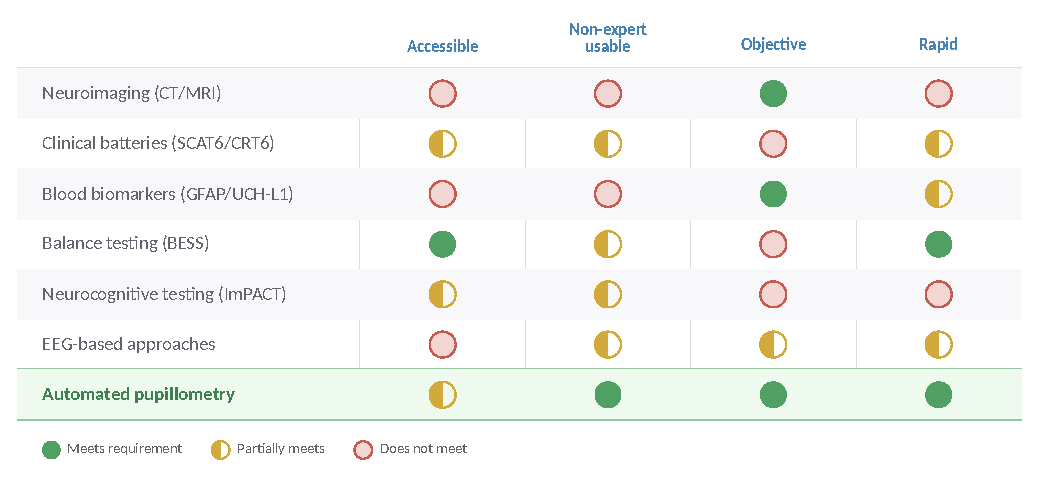
\includegraphics[width=\textwidth]{figures/screening_comparison.pdf}
    \caption{Comparison of candidate mTBI screening approaches against the four requirements identified in \Cref{chapter:introduction}. Automated pupillometry most closely satisfies all four criteria, though most existing commercial implementations remain expensive and clinic-based. This accessibility gap is the engineering problem addressed by this project.}
    \label{fig:screening_comparison}
\end{figure}

\Cref{chapter:introduction} identified four requirements for an effective point-of-injury screening tool: accessible without medical infrastructure, usable by non-experts, objective and cooperation-independent, and rapid. This section evaluates existing diagnostic approaches against these criteria (\Cref{fig:screening_comparison}) to motivate the choice of automated pupillometry.

\textbf{Neuroimaging.} Neuroimaging serves a different clinical purpose to field screening: CT and MRI are used to rule out life-threatening pathology such as intracranial haemorrhage once a patient has reached hospital, not to diagnose \ab{mtbi} at the point of injury~\cite{stiell2001ct, haydel2000ct}. Moreover, conventional imaging is largely insensitive to the pathology of \ab{mtbi}: the majority of patients present with normal CT scans, as diffuse axonal injury produces no visible density changes~\cite{lee2005neuroimaging}. MRI detects abnormalities in approximately 28\% of CT-negative patients~\cite{yuh2013mri}, but most \ab{mtbi} cases remain invisible even on MRI. Advanced diffusion tensor imaging can detect white matter microstructural changes~\cite{palacios2022dti} but remains a research tool. All neuroimaging modalities require hospital infrastructure, specialist operation, and substantial cost.

\textbf{Clinical assessment batteries.} The \ab{scat6} provides structured evaluation combining symptom inventories, cognitive screening, and balance testing, but requires a trained healthcare professional to administer and interpret~\cite{echemendia2023scat6}. The CRT6, designed for non-medical personnel, provides only observational guidance without quantitative metrics~\cite{echemendia2023crt6}. Systematic reviews report highly variable diagnostic performance across assessment components, with sensitivity ranging from 13--92\%~\cite{nelson2013diagnostic}. All such tools depend on either medical training or patient self-report, the latter being vulnerable to symptom minimisation by athletes motivated to continue playing~\cite{meier2015underreporting}.

\textbf{Blood biomarkers.} The FDA-cleared combination of GFAP and UCH-L1 serum biomarkers achieved 97.5\% sensitivity for predicting CT-visible abnormalities, but only approximately 40\% specificity~\cite{bazarian2018blood}. Importantly, these biomarkers are validated for predicting CT findings, not for diagnosing \ab{mtbi} itself. They require venipuncture by trained personnel, laboratory or point-of-care analyser infrastructure, and must be collected within 12 hours of injury. These constraints preclude field deployment by non-medical personnel.

\textbf{Balance and neurocognitive testing.} The Balance Error Scoring System (BESS), commonly used alongside the \ab{scat6}, demonstrates poor sensitivity of only 34\% acutely, declining further over subsequent days~\cite{bell2011bess}. Computerised neurocognitive tests such as ImPACT achieve higher sensitivity (approximately 82\%) but require baseline comparison testing, are vulnerable to deliberate underperformance, and take 20--25 minutes to administer~\cite{schatz2006impact}. Both approaches depend on patient cooperation and physical or cognitive effort.

\textbf{EEG-based approaches.} Quantitative EEG and event-related potential measurements can detect electrophysiological changes following \ab{mtbi}. However, the American Clinical Neurophysiology Society has stated that current evidence does not support the clinical use of quantitative EEG for diagnosing \ab{mtbi}~\cite{nuwer2021qeeg}. Portable systems exist but require electrode application and are sensitive to movement artefact in field environments.

\textbf{Automated pupillometry.} Quantitative measurement of the pupillary light reflex and other oculomotor responses provides objective, involuntary biomarkers that do not depend on patient self-report or cooperation. Automated systems require minimal training to operate, can complete assessment in under one minute, and have demonstrated diagnostic accuracy of 91--96\% with machine learning analysis~\cite{maxin2024smartphone}. Automated pupillometry therefore satisfies three of the four screening requirements directly: it is usable by non-experts (automated measurement and analysis), objective and cooperation-independent (involuntary physiological responses), and rapid (seconds per measurement). However, most existing commercial pupillometers cost thousands of pounds and are designed for clinical facilities, leaving accessibility as an unresolved engineering challenge. This is the gap addressed by this project.

\textbf{Synthesis.} Automated pupillometry is the only reviewed approach that satisfies or partially satisfies all four screening requirements (\Cref{fig:screening_comparison}). The remaining barrier is accessibility: existing systems are expensive and clinic-based. It is also important to note that the highest published accuracy figures derive from machine learning models validated in specific cohorts, and prospective multi-site validation remains necessary. The following section details the oculomotor biomarkers that underpin this approach.


\section{Oculomotor Biomarkers}
\label{sec:bg-oculomotor}

Oculomotor dysfunction is a commonly observed consequence of \ab{mtbi}, with prevalence rates of 65--90\% across multiple studies~\cite{mcdonald2022eye}. This high prevalence reflects the vulnerability of oculomotor control networks to diffuse axonal injury. The distributed neuroanatomical architecture underlying eye movements, spanning from cortex through brainstem to cerebellum, creates multiple points of potential disruption following traumatic injury.

Oculomotor biomarkers offer several advantages over conventional symptom-based approaches. First, oculomotor responses are largely involuntary and autonomic, providing objective measurement independent of patient effort or malingering. Second, oculomotor parameters are quantifiable as continuous metrics amenable to statistical analysis and machine learning. Third, oculomotor testing provides rapid assessment capability (3-4 seconds for pupillary testing, 20-30 seconds for smooth pursuit). Finally, recent technological advances have made oculomotor assessment accessible via low-cost camera systems~\cite{maxin2024smartphone}.

\subsection{Pupillary Light Reflex}

\subsubsection{Mechanism and Pathophysiology}

The pupillary light reflex (\ab{plr}) involves coordinated parasympathetic and sympathetic pathways that regulate pupil diameter in response to changing light conditions. The pathway traverses from retinal photoreceptors through the optic nerve to the pretectal nucleus, then bilaterally to both Edinger-Westphal nuclei in the dorsolateral midbrain. Efferent fibres travel via cranial nerve III to the ciliary ganglion and ultimately innervate the pupil sphincter muscle, producing constriction~\cite{ciuffreda2017plr}.

The extensive anatomical distribution of \ab{plr} pathways creates multiple points of vulnerability to traumatic injury. Diffuse axonal injury affects brainstem structures, particularly the dorsolateral midbrain and upper pons, regions containing the Edinger-Westphal nucleus and sympathetic descending pathways. Shearing forces during head acceleration can disrupt these structures, resulting in altered pupillary dynamics~\cite{bruggeman2020tai}.

\subsubsection{Research Evidence}

Master and colleagues examined \ab{plr} metrics in 98 adolescent athletes with sport-related concussion compared to 134 healthy controls. Using quantitative pupillometry at a median of 12 days post-injury, they found that eight of nine \ab{plr} parameters differed significantly between groups. Concussed athletes demonstrated larger maximum pupil diameter (4.83 mm vs 4.01 mm), faster peak constriction velocity (4.88 mm/s vs 3.91 mm/s), and prolonged recovery time. Maximum pupil diameter and peak constriction velocity achieved \ab{auc} values of 0.78 for discrimination~\cite{master2020pupillary}.

Ciuffreda and colleagues found that 5-8 of 9 \ab{plr} parameters showed statistical differences between \ab{mtbi} and control groups for any given test condition. The most diagnostically useful parameters included constriction latency (194-214 ms in \ab{mtbi} vs 182-199 ms in controls), baseline diameter, response amplitude, and recovery times~\cite{ciuffreda2017plr}.

Recent advances in automated pupillometry with machine learning have demonstrated diagnostic accuracy approaching specialised medical devices. A study of 93 Division I football players achieved 91\% overall accuracy, 98\% sensitivity, and 84.2\% specificity with \ab{auc} of 0.91 using seven \ab{plr} parameters analysed with machine learning models~\cite{maxin2024smartphone}. These results demonstrate the feasibility of accessible, automated \ab{mtbi} screening.

\subsection{Smooth Pursuit Eye Movements}

\subsubsection{Mechanism and Pathophysiology}

Smooth pursuit eye movements maintain visual fixation on moving targets by matching eye velocity to target velocity. Smooth pursuit involves a distributed neural network spanning cortical areas (visual motion processing in area MT/V5, motor planning in frontal eye fields), pontine nuclei serving as relay stations, and cerebellar structures (flocculus and paraflocculus) that generate appropriate motor commands. Cerebellar output projects to the medial vestibular nucleus, which drives extraocular motor neurons controlling eye movement execution~\cite{mcdonald2022eye}.

This extensive pathway traverses multiple white matter tracts susceptible to \ab{dai}, including the corona radiata, internal capsule, pontocerebellar pathways, and cerebellar peduncles. Diffusion tensor imaging studies provide direct evidence of structural damage to smooth pursuit pathways: one study found that 89\% of post-concussion athletes showed abnormal axial diffusivity in at least one white matter tract, with 61\% showing abnormalities specifically in the middle cerebellar peduncle carrying corticopontocerebellar fibres essential for smooth pursuit~\cite{mallott2019cerebellar}.

\subsubsection{Research Evidence}

Within 24-48 hours post-concussion, Division I athletes demonstrated significantly reduced smooth pursuit velocity (14.24±2.31 degrees/second vs 17.86±5.75 degrees/second in controls, p=0.019, Cohen's d=0.83), with increased saccadic amplitude and velocity to compensate for reduced pursuit. These large effect sizes demonstrate clinically meaningful impairment~\cite{murray2019smooth}.

An important enhancement to smooth pursuit assessment involves dual-task paradigms combining eye tracking with concurrent cognitive load. Studies using concurrent working memory tasks (n-back paradigms) have shown substantial improvements in diagnostic discrimination. Baseline smooth pursuit identified 58\% of patients, but adding a concurrent 2-back working memory task increased identification to 79\%. The \ab{auc} for radial variability increased from 0.88 at baseline to 0.946 with cognitive load~\cite{stubbs2018working}.

Smooth pursuit within 7 days of injury shows robust discriminative ability, establishing it as a valuable component of multi-modal assessment~\cite{hunfalvay2021smooth}.

\subsection{Vergence and Near Point of Convergence}

\subsubsection{Mechanism and Pathophysiology}

Vergence eye movements enable binocular vision by coordinating the eyes to converge (move inward) or diverge (move outward) when shifting gaze between near and far targets. Vergence control involves the mesencephalic reticular formation (MRF) located dorsolateral to the oculomotor nucleus, which contains vergence premotor neurons that encode vergence angle and velocity. These neurons project directly to medial rectus motoneurons in the oculomotor nucleus. Cerebellar structures, particularly the caudal fastigial nucleus, also contribute to vergence control~\cite{searle2016vergence}.

Vergence dysfunction in \ab{mtbi} reflects disruption across this distributed network. Rotational acceleration generates focal shear stresses at the mesencephalic and pontine levels, affecting vergence control structures. Convergence insufficiency, the inability to adequately converge the eyes for near work, represents one of the most prevalent oculomotor dysfunctions in \ab{mtbi}~\cite{yaramothu2019vergence, wiecek2021vergence}.

\subsubsection{Research Evidence}

Convergence insufficiency prevalence increases substantially following \ab{mtbi}. Baseline prevalence in the general population ranges from 2-8\%. Post-concussion acute prevalence (<1 month) increases to 35-49\%, representing an 8-84 fold elevation over baseline. Among athletes with chronic concussion-related symptoms, 89\% demonstrate abnormal \ab{npc}~\cite{mucha2014voms, pearce2015npc}.

Clinical assessment using \ab{npc} measurement shows robust diagnostic utility. In concussed patients, \ab{npc} averaged 5.9±7.7 cm compared to 1.9±3.2 cm in controls (mean difference 4.0 cm, p<0.001). Using a clinical threshold of \ab{npc} ≥5 cm, identification rate reached 84\% with \ab{auc} of 0.73. Multivariate models combining \ab{npc} with vestibular-ocular reflex testing and visual motion sensitivity achieved \ab{auc} of 0.89 (95\% CI: 0.84-0.95)~\cite{mucha2014voms}.

Convergence insufficiency correlates significantly with neurocognitive deficits, establishing that vergence dysfunction reflects broader cognitive impairment. Concussed athletes with convergence insufficiency demonstrated significantly worse verbal memory, visual motor speed, and reaction time compared to concussed athletes with normal \ab{npc}. \ab{npc} distance contributed an additional 13.6\% variance in reaction time after controlling for age and symptoms (p<0.001)~\cite{pearce2015npc}.

Prognostic value has been established in multiple studies. Athletes with convergence insufficiency showed 12.3-fold increased odds of prolonged recovery (≥28 days), with mean recovery time of 51.6±53.9 days versus 19.2±14.7 days in the normal \ab{npc} group~\cite{duprey2017convergence}. In emergency department patients, convergence insufficiency scores significantly predicted post-concussion syndrome development, with a multivariate model achieving strong predictive performance (p<0.0001, R²=36\%)~\cite{devani2024convergence}.

\subsection{Rationale for Multi-Modal Assessment}

While each oculomotor biomarker demonstrates diagnostic utility independently, multi-parameter assessment combining PLR, smooth pursuit, and vergence provides superior performance. Different biomarkers may be differentially affected depending on the specific white matter tracts and neural structures damaged in a given patient's injury. Multi-modal assessment increases sensitivity by detecting abnormality when any single parameter is impaired, while maintaining specificity through algorithms that integrate information across parameters. Video-oculography assessment of combined oculomotor parameters achieved 91\% accuracy with 90\% sensitivity and 89\% specificity, while automated multi-parameter pupillometry achieved 91\% accuracy with 98\% sensitivity and 84\% specificity~\cite{kelly2019combined, maxin2024smartphone}.


\section{Engineering Lit Review}
\label{sec:bg-engineering}

\todo{Engineering literature review to be completed.}
